% trabajo desarrollo Demo web R-Tree 
% integrantes 
%Daniel Palomino,Jose Chavez, Vittorino Mandujano,Wilderd Mamani
%----------------------------------

\documentclass[12pt]{article}
\usepackage[margin=1in]{geometry}% Change the margins here if you wish.
\setlength{\parindent}{0pt} % This is the set the indent length for new paragraphs, change if you want.
\setlength{\parskip}{5pt} % This sets the distance between paragraphs, which will be used anytime you have a blank line in your LaTeX code.
\pagenumbering{gobble}% This means the page will not be numbered. You can comment it out if you like page numbers.

%------------------------------------

% These packages allow the most of the common "mathly things"
\usepackage{amsmath,amsthm,amssymb}

% This package allows you to add images.
\usepackage{graphicx}
\usepackage{float}
\usepackage[utf8]{inputenc}
\usepackage{hyperref}
\usepackage{wasysym} %this lets me make smiley faces :-)

%-----------------------------------------------------------------------------------------------------------------------------------
\title{RTREE} % TITULO 
%-----------------------------------------------------------------------------------------------------------------------------------

%integrantes.
\author{Daniel Palomino, \\ Jose Chavez, \\Vittorino Mandujano, \\Wilderd Mamani}

% fecha actulizacion de cada dia
\date{Agosto 15, 2018}

\begin{document}

\maketitle
%-----------------------------------------------------------------------------------------------------------------------------------
\section*{Resumen}  % RESUMEN 
\pagenumbering{arabic}
%-----------------------------------------------------------------------------------------------------------------------------------

El presente reporte abarca la implementación y el funcionamiento de un \textbf{R-Tree}. El \textbf{R-Tree} es una estructura de datos multidimensional usado para metodos de acceso espacial. Algunos ejemplos de estas estructuras son: sistemas de coordenadas geográficos, rectángulos o polígonos. Esta  estructura es de mucha importancia por las aplicaciones teóricas y prácticas en el mundo real, como por ejemplo ``Encontrar todos los museos en un radio de dos kilómetros alrededor de la posición actual''.La idea principal de esta estructuda de datos y la descripción será descrita así como la implementación en un demo web con una interface gráfica. El demo implementado nos permite dibujar puntos y polígonos con el mouse en un entorno canvas descrito en este reporte. Adicionalmente se presentan los resultados obtenidos, las limitaciones así como las conclusiones y trabajos futuros.


\paragraph{Documentación adicional:} 
\begin{enumerate}
\item GitHub: \url{https://github.com/AED-RTREE/rtree}. 
\item Video Youtube: \url{https://www.youtube.com/watch?v=a6DZWz91xNo}
\end{enumerate}
%-----------------------------------------------------------------------------------------------------------------------------------
\section*{Descripción Conceptual del R-Tree} % DESCRIPCION CONCEPTUAL
%-----------------------------------------------------------------------------------------------------------------------------------
El \textbf{R-Tree} fue creado por Antonin Guttman el año 1984. Puede considerarse como una generalización del B-Tree, una estructura de datos unidimensional. El \textbf{R-Tree} es idóneo para representar objetos en un espacio multidimensional, ergo para figuras en el plano.\\

El \textbf{R-Tree} es un árbol balanceado donde todos sus objetos están en las hojas, encerradas por una región. Para el caso bidimensional, los objetos son puntos y polígonos delimitado por un cuadrilátero. Los nodos de la parte superior están relacionados con las regiones que contienen a dichos objetos. Cada nodo posee una cantidad bien diefinida de regiones y en cada región hay un nodo. La forma del árbol resultante podemos contemplarla en la figura 1.\\

\begin{figure}[!h]
\centering
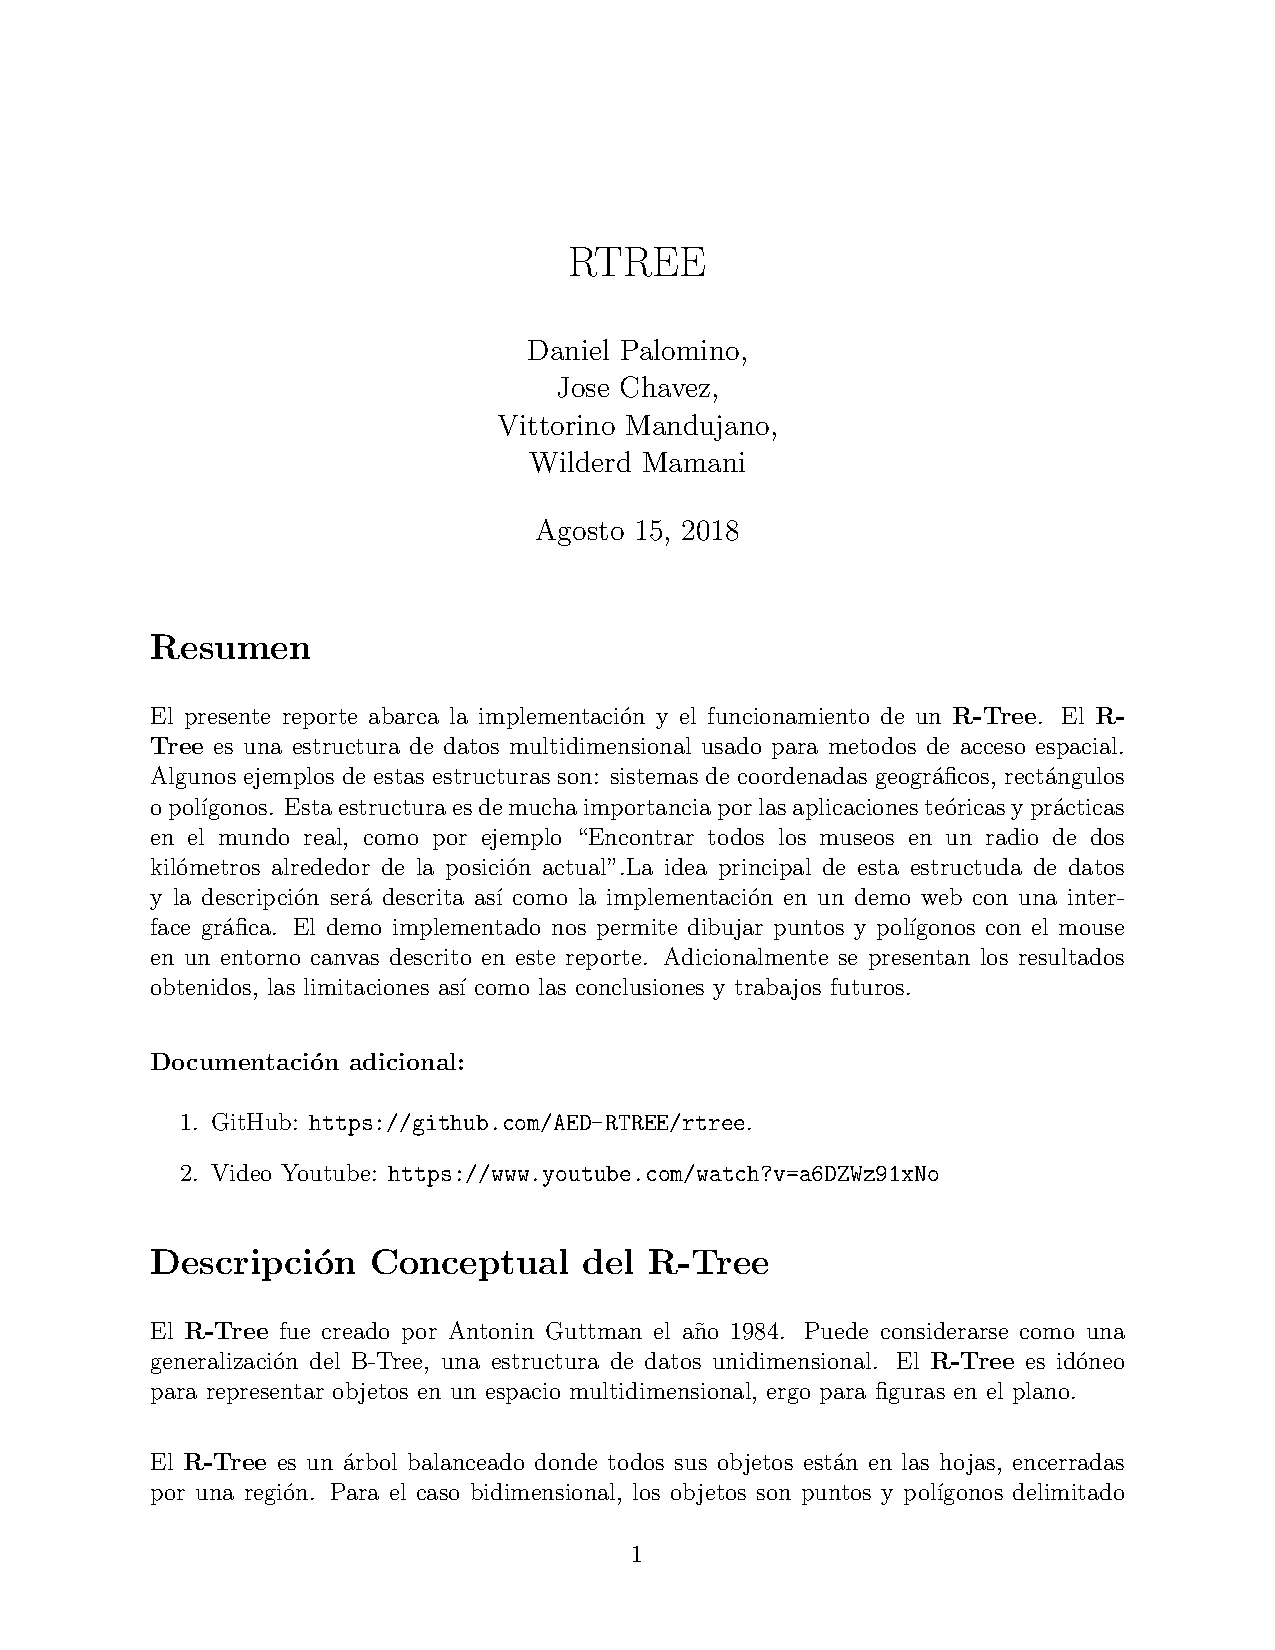
\includegraphics[width= 0.6 \textwidth]{images/rtree.png}
\centering
\caption{Ejemplo de un RTree.}
\end{figure}

Cada nodo tiene una cantidad mínima $m$ y máxima $M$ de regiones. Una cantidad fuera de dicho rango ocasiona, para un exceso de regiones, un split o división del nodo. Por otra parte, una cantidad menor al rango ocasiona una unión de estos. La cantidad mínima de regiones suele ser cerca de la mitad de la cantidad máxima de regiones, la única excepción a dicha regla ocurre con el nodo raíz que puede tener un minimo de 2 regiones.\\

Tomando por ejemplo el caso basado en los datos de la figura 2. Si lo representamos con un R-Tree con un $m=2$ y un $M=5$
tendríamos un árbol como en la figura 3.

\begin{figure}[!h]
\centering
\includegraphics[width= 0.3 \textwidth]{images/table.png}
\centering
\caption{Ejemplo de base de datos alumno y creditos}
\end{figure}


\begin{figure}[!h]
\centering
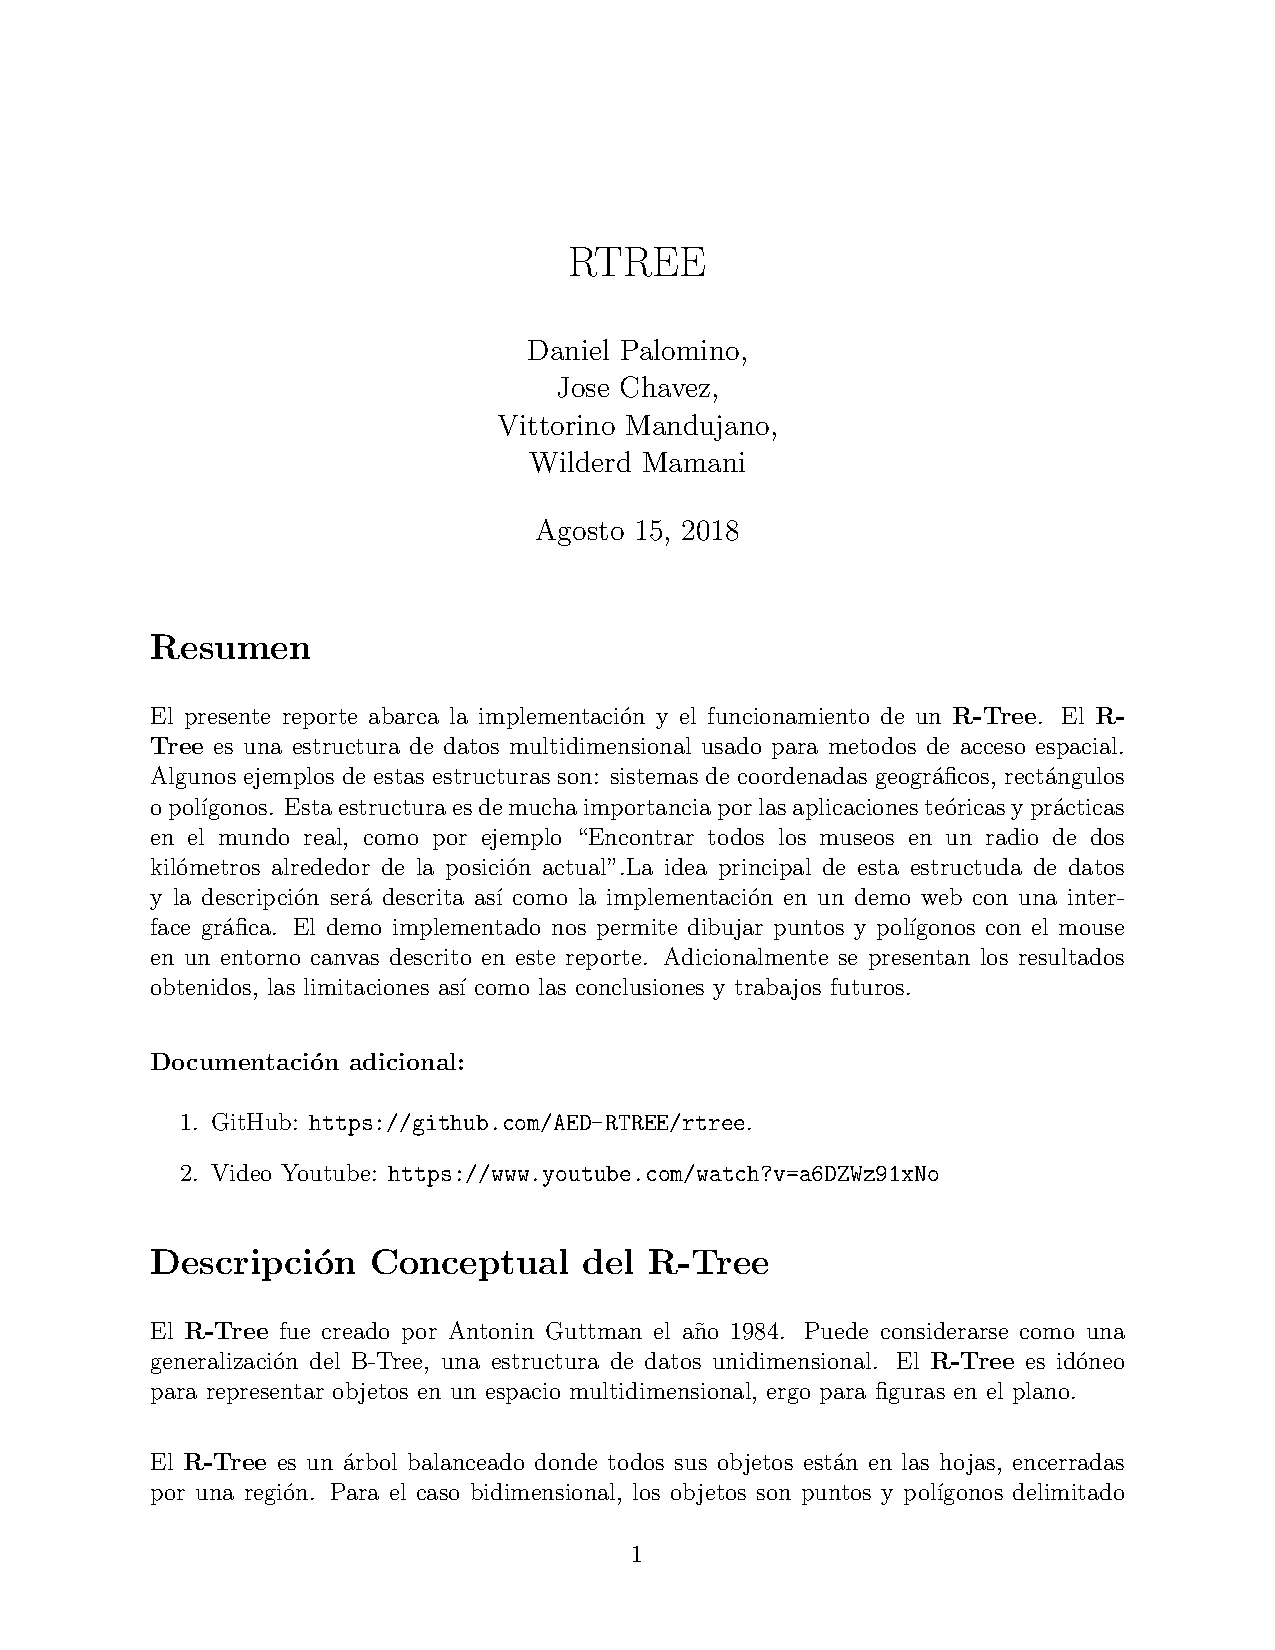
\includegraphics[width= 0.6 \textwidth]{images/rtree.png}
\centering
\caption{RTree correspondiente a los datos de la Fig. 2}
\end{figure}

Podemos contemplar que la raíz esta formada por las regiones $R1$ y $R2$. Estas a su vez apuntan a los nodos del siguiente nivel. El nodo que apunta $R1$ contiene las regiones $R3$, $R4$ y $R5$ y el nodo que apunta $R2$ contiene las regiones $R6$ y $R7$. Este árbol podemos representarlo gráficamente en el plano tal como se muestra en la figura 4.


\begin{figure}[!h]
\centering
\includegraphics[width= 0.6 \textwidth]{images/rectangules.png}
\centering
\caption{La grafica muestra el diagrama de los rectangulos de la base de datos ejemplo}
\end{figure}

Como toda estructura de datos, en el R-Tree podemos realizar las operaciones elementales: Búsqueda, Inserción y Eliminación.

\paragraph{Busqueda:} la busqueda en el R-Tree funciona de manera similar al B-Tree, tal y como este ultimo el arbol va descender desde la raiz, en los arboles R se almacenan rectangulos quienes se pueden sobreponer, por que todos los rectangulos tienen que ser visitados.
Sea T la raiz de un r-tree. ahora vamos a buscar todos los indices guardados de quienes los rectangulos un rectángulo de búsqueda especificado S,
\begin{itemize}
    \item si T no es una hoja, entonces aplicamos la busqueda en cada hijo de quienes la raiz esta apunta por el puntero hijo y este se superpone con $S$.
    \item Si T es una hoja, retorna todas la entradas que se superponen con $S$ como el conjunto resultante.
\end{itemize}

un ejemplo de acuerdo a nuestro ejemplo base seria graficamente.

\begin{figure}[!h]
\centering
\includegraphics[width= 0.6 \textwidth]{images/search.png}
\centering
\caption{Ejemplo de busqueda de estudiantes.}
\end{figure}

En el ejemplo anterio queremos encontrar todos los estudiantes que estan en el secto semestre o mas y que tienen entre 20 y 65 creditos, ademas podemos ver que R1 se superponecon la consulta del rectangulo $S$,sin R2, asi que vamos a buscar en R1, en el siguiente paso R4 y R5 esta superpuestos con $S$ en estos rectangulo de busqueda encontramos que C esta dentro de R4 y E,K estan dentro de R5, asi el resultado es ${C,E,K}$

\paragraph{Inserción:} Se tiene un objeto (polígono o punto) y se delimita por un MBR. Luego se realiza el proceso de búsqueda para añadirlo en las regiones y nodos correspondientes. Después se tiene que verificar si el árbol todavía cumple las condiciones impuestas por $m$ y $M$. Se realiza dicha prueba por el camino que fue descrito por la búsqueda, pero en orden inverso.

\paragraph{Eliminación:} Para eliminar un objeto se realiza la búsqueda del objeto. Una vez encontrado este es eliminado y se revisa los nodos por los que se recorrió en la búsqueda para cumplir las condiciones de $m$ y $M$.
%-----------------------------------------------------------------------------------------------------------------------------------
\section*{Implementacion del Demo web} % DESCRIPCION BREVE DEMO WEB
%----------------------------------------------------------------------------------------------------------------------------------

Para la implementación del presente Demo Web, se usó una arquitectura de 3 capas:

\begin{enumerate}
\item La Aplicación Web, desarrollado en un entorno canvas de html5 y Javascript para la funcionalidad y manipulación de las etiqueta.

\item La conectivad basada en sockets, siendo el servidor construído sobre c++ con métodos de bajo nivel implementados sobre c con librerías nativas de sistemas tipo unix como socket.h, y el ciente construído sobre python.

\item El Aplicación RTree, que almacena los objetos insertados por el usuario, para posteriormente poder realizar consultas sobre él.
\end{enumerate}

En la $Figura [6]$ se puede apreciar el flujo de información a través de estos 3 níveles o capas.

\begin{figure}
\centering
\includegraphics[width= 0.6 \textwidth]{images/demo.png}
\centering
\caption{Diagrama general del demo web}
\end{figure}

\subsection*{Conectividad }

La capa de conectividad está compuesta por 2 partes:

\begin{enumerate}
\item El Socket Servidor, implementado en c++ usando la librerías $socket.h$ nativa de sistema tipo UniX.
\item El Socket Cliente, implementado en python 2.7 usando el módulo $socket$ de su libería estándar.
\end{enumerate}

Para un mejor manejo de la información entre ambos procesos se diseñó un protocolo simple para el envío de los objetos insertado y las diferentes consultas posibles (Range, Nearest) y una respuesta que permita saber si la información fue envíada y recibida de manera correcta, y prevenir de esta manera errores por pérdida de datos.

En la $Figura [7]$ se muestra un ejemplo de algunos casos usando este protocolo.

\newpage

\begin{figure}
\centering
\includegraphics[width= 0.4 \textwidth]{images/trama1.png}
\centering
\caption{Trama de consultas y respuestas del TCPServer}
\end{figure}

El funcionamiento es bastante simple, se construye un $string$ usando el $comando$ envíado más los objetos a enviar, todo separado por palotes $(|)$.

Siendo la estructura general de envío desde el cliente de la siguiente manera:

\[
    \textup{COMMAND} |N|X_1|Y_1|X_2|Y_2 \dots | \textup{END}
 \]
 
 Donde:
\begin{enumerate}
\item \textbf{N} es el numero de puntos del objeto a enviar.
\item Finalmente, las coordenadas de los puntos del objeto en orden $(x_1,y_1)\dots (x_c,y_C)$.
\end{enumerate}

Y la respuesta del servidor:

 \[
    \textup{COMMAND} |N|M_1||X_1|Y_1|X_2|Y_2 \dots | \textup{END}
 \]

Donde:
\begin{enumerate}
\item \textbf{N} es el número de niveles del árbol.
\item \textbf{M} es el número de MBRs de cada nivel.
\item seguido del número de \textbf{C} puntos a enviar por MBR.
\item Finalmente, coordenadas de los puntos del MBR en orden $(x_1,y_1)\dots (x_c,y_C)$.
\end{enumerate}
\newpage

%---------------------------------------------------------------------------------
%\subsection*{)}
\paragraph*{Aplicación Web}~\\\\
La implementan web fue desarrollada con la tecnología HTML5 y Javascript para la manipulación de las etiquetas html y el entorno gráfico, en el cual se pueden insertar polígonos y los puntos, para esto se utilizó canvas-html y para crear la aplicación web se utilizó Flask, un framework de Python. Además se aprovechó el módulo "socket" de la librería estándar para la conexión con el servidor. De este modo logramos la conexión con nuestro código fuente desarrollado en c++, los detalles de instalación y ejecución están detallados en un repositorio GitHub.\\

Aplicativo cuenta con la función INSERT, que nos permite ingresar puntos y poligons, dentro de un recuadro de 854x480 pixeles, permitiendo visualizar en tiempo real los MBRs generados con su respectiva etiqueta y color. Las etiquetas siguen un orden específico de acuerdo al nivel, empezando desde la vocal 'A' y adjuntando el número respectivo de MBR en el nivel, del mismo modo los colores ayudan a diferenciar los niveles.\\

La función RANGE permite encontrar los elementos dentro de un rectángulo, y resaltando los elementos encontrados en color verde. Por ultimo se tiene la función NEAREST que nos permite encontrar los elementos mas cercanos a un punto, previamente ingresando un valor (k), en otras palabras encuentra los k-elementos más cercanos a un punto. Los elementos son resaltados del mismo modo, con un color verde y una respectiva linea que permite visualizar de una mejor manera a que elementos se refiere.\\\\
Por último se tiene la función DELETE ALL que elimina todos los poligonos y puntos y por consecuencia todos los MBRs generados.\\\\
Cada una de estas funciones fueron diseñadas en Javascript, estas funciones envían los datos a un programa en Python que se encarga de empaquetar los datos y enviarlos al Servidor con la ayuda de la librería 'socket' de Python. Este programa también recibe los datos del servidor y se encarga de modificar los valores en Javascript para luego dibujarlos dentro del canvas y asi poder visualizar las diferentes figuras. 


\newpage
\begin{figure}
\centering
\includegraphics[width= 1.0 \textwidth]{images/nearest.png}
\centering
\caption{Ejecutando la funcion K-Neasrest}
\end{figure}



\subsection*{Implementacion R-Tree: } 
\paragraph{ Estructura del R-Tree: } El R-Tree fue implementado con la clase R-Tree y varias estructuras, quienes son: Rect, Node, Branch, ListNode y PartitionVars.\\
\begin{itemize}
\item Nodo: La clase nodo, la clase RTree tiene por defecto uno y es la raíz\\
\item Region: corresponde a las regiones que poseen los nodos. Las regiones tienen un puntero a Nodo.\\
\item Mbr: Corresponde al MBR de las regiones, todas las Regiones tienen uno.\\
\item ListNode: Lista que contienen nodos y sirven para grabar el recorrido de la búsqueda.\\
\item PartitionVars:  Estructura que facilita el split de los nodos .
\end{itemize}
\paragraph{Descripción del Código :} Consta de 5 funciones principales correspondientes a insertar,eliminar todos, búsqueda y busqueda de los objetos cercanos. Y de funciones complementarias que son 34.

%-----------------------------------------------------------------------------------------------------------------------------------
\section*{Resultados} % RESULTADOS OBTENIDOS
%-----------------------------------------------------------------------------------------------------------------------------------
En este informe detallamos la implementación de un demo web, con visualización grafica de los poligonos con regiones sombreadas y puntos, a los cuales podemos hacer consultas usando el mouse como las regiones a un rectángulo y los puntos mas cercanos a un punto k elegido.
El demo muestra la partición a medida que se va insertando mas poligonos, asi como las regiones MBR que contienen a estas de tal manera que la respuesta del algoritmo R-Tree implementado en c++ es visualizada en la pantalla canvas del demo. Además podemos ver de manera interactiva los puntos mas cercanos, atraves de una linea a todos los puntos mas cercanos del punto elejido con el mouse y las figuras coloreadas a una región (rectángulo) seleccionado por el mouse.
Finalmente podemos ver los puntos en coordenadas que usamos con el mouse en cada elección de los botones, de tal manera que podemos ver los puntos elegidos en cada click. Asi en el demo web se puede apresiar de manera visual la estructura de datos espacial R-Tree.

%-----------------------------------------------------------------------------------------------------------------------------------
\section*{Limitaciones} % LIMITACIONES  DEL DEMO WEB 
%-----------------------------------------------------------------------------------------------------------------------------------
\begin{itemize}
\item El presente proyecto de aplicación web de la estructura de datos multidimencional R-Tree ha sido desarrollada para un caso particular de poligonos y puntos, por fines de estudio y aplicacion práctica de la teoria del algoritmo.
\item El Algoritmo modulo cuenta con un modulo split utilizado para la particion el cual cuenta con uno de las muchas formas de particion con fines practicos se utilizo la particion cuadratica.
\item La ejecución e instalacion del presente proyecto necesita un sistema ubuntu del parte del servidor por la dependencia de las librerias.
\end{itemize}

%-----------------------------------------------------------------------------------------------------------------------------------
\section*{Trabajos Futuros} % TRABAJOS FUTUROS 
%-----------------------------------------------------------------------------------------------------------------------------------
\begin{itemize}
\item Implementar la aplicación solo en Javascript de tal modo que se pueda ejecutar las funciones de forma continua y ver los MBRs en tiempo real.
\item Visualizar el árbol completo de forma dinámica.
\item Permitir la configuración de los parámetros del R-Tree desde la aplicación web.
\item Implementar la aplicación para la ejecucion del demo web y eliminar la dependencia del sistema operativo.
\end{itemize}

%-----------------------------------------------------------------------------------------------------------------------------------
\section*{Conclusiones} % CONCLUSIONES 
%-----------------------------------------------------------------------------------------------------------------------------------
%-----------------------------------------------------------------------------------------------------------------------------------
Este proyecto muestra la implementación de un R-Tree en un vizualizador web canvas de poligonos y puntos, para fines netamente aplicativos de la estructura de datos R-Tree,a pesar que nuestro demo muestra los puntos pequeños, añadimos una vizualización mas interactiva de acuerdo a movimiento del mouse, por lo cual podemos mostrar como funciona el k nearest. Por otro lado la implementación de la parte del servidor se realizó con libreria unix , por lo que recomendamos usar linux ubuntu para test del demo, debido a la dependencia que encontramos en la librerias antes mencionada en el lado del servidor de extension cpp. 
\section*{Referencias}  % REFERENCIA Y BIBLIOGRAFIA
%-----------------------------------------------------------------------------------------------------------------------------------
\begin{enumerate}
\item  {\it Spatial Data Structures class}; Laura Toma; \\
\small{\url{http://www.bowdoin.edu/~ltoma/teaching/cs340/spring08/Papers/Rtree-chap1.pdf}}
\item {\it R-Trees: Theory and Applications};Y. Manolopoulos; A. Nanopoulos; Y. Theodoridis (2006) 
\item  {\it R-Tree concept }; wikipedia the free enciclopedia; 
\small{\url{https://en.wikipedia.org/wiki/R-tree}}
\item  {\it R-trees: a dynamic index structure for spatial searching}; Dan Hanmore 	Antonin Guttman 	University of California, Berkeley; 
\item  {\it R-Tree concept }; wikipedia the free enciclopedia; 
\small{\url{https://en.wikipedia.org/wiki/R-tree}}
\item {\it The Priority R-tree}; \url{http://www.win.tue.nl/~mdberg/Papers/prtree.pdf}
\end{enumerate}


%-----------------------------------------------------------------------------------------------------------------------------------
\section*{Distribución de trabajo} % DESCRIPCION 
%-----------------------------------------------------------------------------------------------------------------------------------

\begin{itemize}
\item \textbf{Daniel Palomino:}  Socket-Server, RTree.
\item \textbf{José Chávez:}  Aplicación Web, Socket-Cliente.
\item \textbf{Vittorino Mandujano:}  RTree.
\item \textbf{Wilderd Mamani:}  Aplicación Web.
\end{itemize}
\end{document}
